\documentclass{article}
\usepackage[margin=1in]{geometry}
\usepackage{stmaryrd}
\usepackage{amssymb}
\usepackage{tikz}
\usepackage{ stmaryrd }
\usetikzlibrary{positioning}


\title{Interaction Diagram - Get Portfolio}
\author{ Adam Hammes }

% no page number at bottom
\pagenumbering{gobble}

\begin{document}
\maketitle

\begin{center}

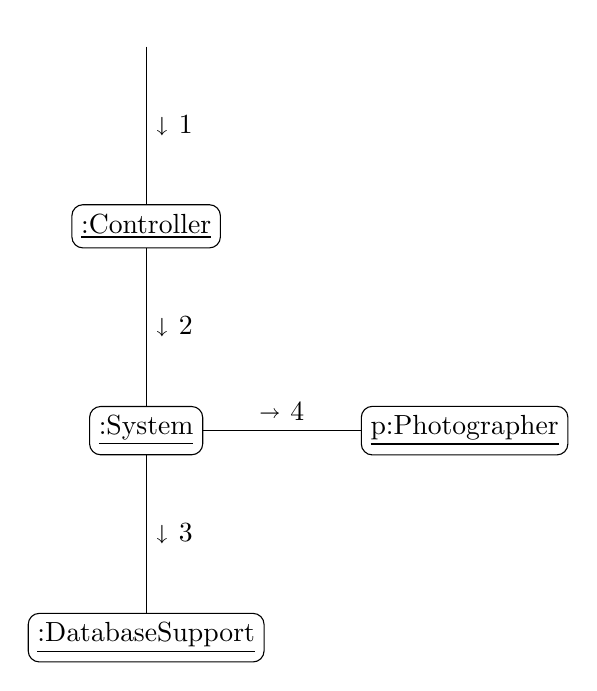
\begin{tikzpicture}[
  auto,
  block/.style = {
    rectangle,
    draw=black,
    align=center,
    rounded corners
  },
  multiple/.style = {
    rectangle, draw, rounded corners, fill= white,
    text width=9em, align= center,
    copy shadow = {
      ,fill=white, draw=black,
      shadow xshift=0.5mm, shadow yshift=-0.5mm
    }
  }
]
\node[] (start)  {};
\node[block, below=2cm of start] (controller) {\underline{:Controller}};
\node[block, below=2cm of controller] (system) {\underline{:System}};
\node[block, below=2cm of system] (db)  {\underline{:DatabaseSupport}};
\node[block, right=2cm of system] (photographer) {\underline{p:Photographer}};

\draw (start) -- (controller) node[midway]{$\shortdownarrow$ 1};
\draw (controller) -- (system) node[midway]{$\shortdownarrow$ 2};
\draw (system) -- (db) node[midway]{$\shortdownarrow$ 3};
\draw (system) -- (photographer) node[midway]{$\shortrightarrow$ 4};


\end{tikzpicture}

\vspace{0.5cm}

\begin{enumerate}
  \item \texttt{l:=getPortfolio(name:String):list<Image>}
  \item \texttt{l:=getPortfolio(name:String):list<Image>}
  \item \texttt{p:=getPhotographer(name:String):Photographer}
  \item \texttt{l:=getImages():list<Image>}
\end{enumerate}
\end{center}

\end{document}
